\section{System agentowy}
%%%% OPIS NARZĘDZI - plusy i minusy
Na rys. \ref{fig:actor} został umieszczony schemat stworzonej przez zespół architektury systemu agentowego.
\begin{figure}[!htb]
\centering
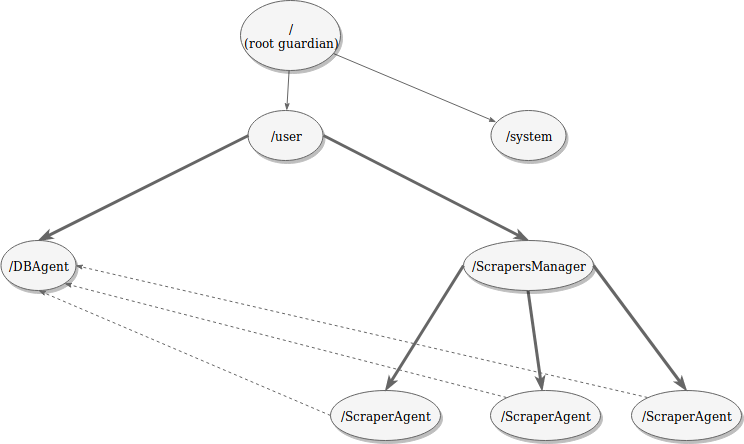
\includegraphics[width=1.0\textwidth]{./pict/actors.png}
\caption{Schemat wdrożonego systemu zgodnie z architekturą Akka}
\label{fig:actor}
\end{figure}

\par Przy czym strzałki pogrubione oznaczają podległość agentów (aktorzy przy końcu strzałki są ''dziećmi'' aktorów z początku strzałki), natomiast dodatkowe strzałki przerywane oznaczają kierunek wysyłania wiadomości do agentów.

\par Poszczególni agenci w systemie różnią się między sobą zadaniami:
\begin{itemize}
	\item \texttt{DBAgent} - pełni zadania agenta mającego bezpośredni dostęp do bazy danych, w której składowane są artykuły. Obsługuje on dwa typy otrzymywanych wiadomości:
     \begin{itemize}
      \item \textbf{SaveArticles} - wiadomość od ScraperAgenta, zlecająca zapisanie do bazy danych listy artykułów
      \item \textbf{SaveArticle} - wiadomość od ScraperAgenta, zlecająca zapisanie do bazy danych pojedynczego artykułu.
     \end{itemize}
                                                                                                                                    	\item \texttt{ScrapersManager} - agent pełniący obowiązki menedżera ScraperAgentów. Przechowuje on mapę referencji do nich, tworzy je oraz cyklicznie zleca im przeglądanie artykułów ze stron. Agent ten obsługuje dwa typy wiadomości:
     \begin{enumerate}
      \item \textbf{OrderScrapping} - wiadomość, którą agent wysyła sam do siebie co pewien określony czas (ustawiony z wykorzystaniem schedulera Akki), a która powoduje wysłanie do każdego zarejestrowanego w nim ScraperAgenta wiadomości typu \textbf{Scrap}
      \item \textbf{CreateScraperAgent} - wiadomość od głównego agenta systemu (\textbf{user}), która zleca utworzenie ScraperAgenta mającego odpowiadać, za przeglądanie strony kanału RSS o określonym adresie URL.
     \end{enumerate}
                                                                                                                                    	\item \texttt{ScraperAgent} - typ agenta odpowiedzialnego za przeglądanie danego kanału RSS, ekstrakcję nowych artykułów, ich wektoryzację oraz wysłanie ich do \texttt{DBAgenta} celem zapisu w bazie danych. Obsługuje on jeden typ wiadomości:
     \begin{enumerate}
      \item \textbf{Scrap} - wiadomość od ScrapersManagera, która zleca przejrzenie kanału RSS, pobranie nowych artykułów, ich wektoryzację i wysłanie do zapisu w bazie danych.
     \end{enumerate}
     Agent przechowuje informację o tym, kiedy nastąpił ostatni pobór danych z kanału RSS, za który odpowiada i na tej podstawie filtruje artykuły z kanału tak, aby nie wysyłać do zapisu artykułów które już istnieją w bazie danych. Za pomocą obiektu \texttt{ScraperHttpService} agent ten komunikuje się z modułem analitycznym wykorzystującym algorytm doc2vec, dzięki któremu następuje wektoryzacja artykułu. Artykuł w pełnej formie (obejmującej treść, adres pobrania, datę publikacji i postać wektorową) zostaje wysłany wraz z wiadomością \textbf{SaveArticle} do \texttt{DBAgenta}.

\end{itemize}

\par System ten został wykonany z użyciem popularnego dla takich celów frameworku Akka oraz języka Scala.

W stworzonym przez zespół systemie część agentów może działać w innych węzłach niż pozostałe. Dzięki wykorzystaniu biblioteki \texttt{Akka Remoting}, zespół przetestował umieszczenie osobno agenta ScrapersManager oraz wszystkich agentów typu ScraperAgent.

\subsection{Język Scala}

\par Framework Akka umożliwia implementację systemów agentowych z wykorzystaniem dwóch możliwych języków - Java oraz Scala. Oba bazują na maszynie wirtualnej Javy, natomiast znacznie różnią się od siebie wykorzystywanym paradygmatem programowania - Java jest językiem typowo obiektowym, podczas gdy Scala umożlwia zarówno korzystanie z paradygmatu obiektowego, jak i funkcyjnego. Ze względu na potencjalne korzyści wynikające z użycia jej, zwięzłość kodu oraz lepsze przystosowanie do założeń systemu obiektowego (takich jak asynchroniczność), zespół, pomimo braku znajomości języka na początku realizacji projektu, zdecydował się na implementację wykorzystującą Scalę.

\par Język Scala okazał się być dla większości członków zespołu językiem trudnym do opanowania o wysokim wymaganym progu wiedzy wejściowej. Pomimo iż dwóch członków zespołu znało paradygmat programowania funkcyjnego z innych języków programowania takich jak Haskell, rozbudowana składnia Scali była na początku trudna do opanowania.

\par Końcowy efekt w postaci zaimplementowanego projektu udowodnił jednakże, iż opanowanie tego języka było warte czasu przeznaczonego na nie. Scala umożliwia korzystanie z paradygmatu funkcjonalnego w sposób, który pomaga w implementacji zamiast nastręczać problemów (co zdarza się w przypadku języków czysto funkcjonalnych, takich jak Haskell). Jej wielką zaletą jest również możliwość korzystania z klas Javy, co umożliwiło zespołowi korzystanie z popularnych bibliotek służących do przetwarzania kanałów RSS i parsowania stron internetowych. Mechanizmy typowe dla języków funkcyjnych, takie jak ''match expressions'', pozwoliły wydatnie zredukować ilość kodu konieczną do implementacji systemu. Cała architektura agentowa zaimplementowana przez zespół przy użyciu Scali zajęła zaledwie 240 linii kodu. Jest on również czytelny i łatwo modyfikowalny.

\par Scala okazała się jednakże nie być właściwym narzędziem jeśli chodzi o stworzenie systemu ORM (ang. \textit{object-relational mapping}). Biblioteka Slick, którą zespół wykorzystał do tego celu, dostarczyła wielu trudności w implementacji.

\subsection{Framework Akka}
\par W celu zrealizowania systemu agentowego zespół zdecydował się wykorzystać framework Akka. Decyzja ta podyktowana była chęcią wykorzystania popularnego w tym zakresie frameworku i stworzenia systemu wykorzystującego wszystkie zalety systemów agentowych - możliwość budowy relatywnie nieskomplikowanych w implementacji systemów, które jednocześnie będą wydajne, łatwo rozszerzalne i rozproszone.
\par Nauka frameworka na podstawie istniejącej dokumentacji była czasochłonna. Dokumentacja zamieszczona na stronie Akki skupia się na zaprezentowaniu zalet korzystania z systemu aktorowego pomijając jednakże szczegóły implementacyjne - prezentuje jedynie dwa przykłady prostego systemu, opisując go w sposób dość rozwlekły.
Bez wykorzystania źródeł zewnętrznych, w tym przykładowych systemów zaimplementowanych z wykorzystaniem tej biblioteki, niemożliwe byłoby na przykład zaimplementowanie systemu rozproszonego z wykorzystaniem biblioteki Akka Remote.
\par Implementacja systemu agentowego ujawniła jednak wszystkie zalety frameworka Akka. Po zapoznaniu sie w dokładny sposób z dokumentacją była ona szybka i nie pociągnęła za sobą znaczących modyfikacji aż do końca projektu, co należy zawdzięczać również przemyślanej uprzednio strukturze systemu.
\par Wielką zaletą frameworka okazała się łatwość rozbudowywania i rozpraszania aplikacji. Zmiana aplikacji z wersji lokalnej na rozproszoną wymagała niemal wyłącznie zmiany w plikach konfiguracyjnych oraz sposobie adresowania aktorów.
\par Również rozszerzenie zakresu analizowanych kanałów RSS okazało się być bezproblemowe. W początkowej wersji systemu analizowane były jedynie kanały RSS o różnej tematyce pochodzące z serwisów informacyjnych BBC oraz CNN. W celu powiększenia zbioru testowego do rozsądnej liczby artykułów, zostały zaimplementowane również parsery takich mediów jak:
\begin{itemize}
	\item Reuters
	\item Washington Times
	\item New York Times
	\item The Guardian
\end{itemize}
Umożliwiło to zwiększenie bazy danych artykułów ze 137 pozycji do niemal 500, pociągając za sobą niecałą godzinę pracy.
\par Możliwość łatwej budowy systemów rozproszonych oraz prostego odwzorowania zaplanowanej architektury w kodzie należą do największych zalet Akki dostrzeżonych przez zespół. Cechy te sprawiają, iż decyzję o implementacji z wykorzystaniem tego frameworka należy określić jako zdecydowanie pozytywną.
\par Istnieją jednakże również negatywne strony takiej decyzji. Systemy agentowe nie należą do najpopularniejszych, co sprawia, że wsparcie społeczności dla frameworka Akka czasami okazywało się niewystarczające. Zespół napotkał duże problemy przechodząc od wersji lokalnej projektu do wersji rozproszonej ze względu na niejednoznaczne komunikaty o błędach. Zostały one jednak szybko pokonane i trudności takie nie przeważają zalet wykorzystania zarówno architektury agentowej, jak i konkretnego frameworka w postaci Akki.

\subsection{Schemat pobierania wiadomości}

Agenty odpowiedzialne za pobieranie oraz parsowanie artykułów, uruchamiane są 
regularnie.
Do pobierania danych z kanału RSS wykorzystano bibliotekę 
\texttt{ROME}, która dla zadanego adresu url pobiera tak zwany \texttt{feed}. Następnie za pomocą narzędzia \texttt{jsoup} 
pobierane oraz parsowane są treści każdego artykułu. 
Następnie treść każdego artykułu poddawany jest wektoryzacji w module NLP. W kolejnym kroku najważniejsze informacje o artykule:
\begin{itemize}
\item adres strony z której został pobrany,
\item strona z której został pobrany,
\item text artykułu,
\item data publikacji,
\item tagi,
\item oraz wektor zwrócony przez moduł NLP,
\end{itemize}
są zapisywane w bazie danych (rys. \ref{fig:db}).

\begin{figure}[ht!]
\centering
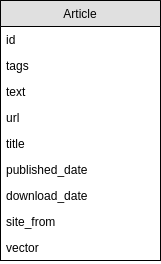
\includegraphics[height=0.3\textheight, width=0.3\textwidth]{./pict/db.png}
\caption{Schemat bazy danych}
\label{fig:db}
\end{figure}